\documentclass{article} 
\usepackage{tikz} 
\usepackage{multicol}
\usepackage{hyperref} 
\usepackage[a4paper]{geometry}
\usepackage{fancyhdr}
\pagestyle{fancy} 
\lhead{Ladungen}
\rhead{August 2025}
\begin{document}
 
\section{Ladungen}
Stoffe können unterschiedlich, entweder \emph{positiv} oder \emph{negativ}, geladen sein. Haben zwei Stofffe die gleiche Ladung, sei es dass beide positiv oder beide negativ sind, so sind diese \emph{gleichnamig} und stoßen sich ab. Ist hingegen ein Stoff positiv und der andere negativ, so sind sie \emph{ungleichnamig} zueinander und ziehen sich an. Die \hyperref[Ladung von Elektronen]{Ladung von Elektronen} ist negativ. \newline
Die Ladung wird mit dem Formelzeigen $Q$ angegeben und in der Einheit $C$, Coulomb, gemessen. 
 
\begin{multicols}{2} 
 \raggedcolumns % fixed heights
 \subsection{Influenz}
 Influenz beschreibt dass bei elektrischen Leitern alle frei beweglichen Elektronen vom einer externen positiven Ladung angezogen beziehungsweise von einer negativen Ladung abgestoßen werden. Durch das Elektronengefälle beider Seiten des Leiters werden diese auch entsprechend aufgeladen.
 \begin{center}
  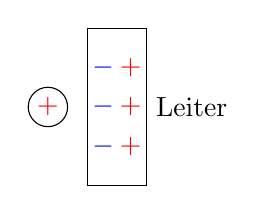
\begin{tikzpicture}
   \draw (0, 0) circle (0.25cm);
   \draw (0, 0) node[red] {$+$};
 
   \draw (0.5, 1) rectangle (1.25, -1); 
   \draw (1.25, 0) node[right] {Leiter};
   \draw (0.7, 0.5) node[blue] {$-$}; 
   \draw (0.7, 0) node[blue] {$-$};  
   \draw (0.7, -0.5) node[blue] {$-$};  
   \draw (1.05, 0.5) node[red] {$+$}; 
   \draw (1.05, 0) node[red] {$+$};  
   \draw (1.05, -0.5) node[red] {$+$}; 
  \end{tikzpicture} 
 \end{center}
 \columnbreak
 \subsection{Polarisation}
 Polarisation beschreibt dass die Elektronen innerhalb der Atome von Isolatoren sich in der Atomülle der Umgebungsladung nach ausrichten können. Dies passiert, weil es in Isolatoren keine frei beweglichen Elektronen gibt. Hier kommt es zu keinem relevanten Elektronengefälle und keiner Ladung.
 \begin{center}
  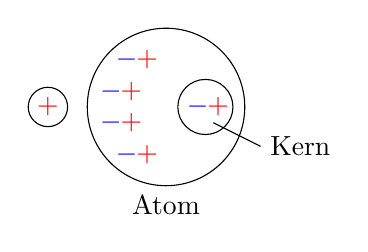
\begin{tikzpicture}
   \draw (0, 0) circle (0.25cm);
   \draw (0, 0) node[red] {$+$};
   
   \draw (1.5, 0) circle (1cm);
   \draw (1.5, -1) node [below] {Atom};
 
   \draw (1, 0.6) node[blue] {$-$} node[red, right] {$+$};  
   \draw (0.8, 0.2) node[blue] {$-$} node[red, right] {$+$};   
   \draw (0.8, -0.2) node[blue] {$-$} node[red, right] {$+$};  
   \draw (1, -0.6) node[blue] {$-$} node[red, right] {$+$};  
 
   \draw (2, 0) circle (0.35cm);
   \draw (1.9, 0) node[blue] {$-$} node[red, right] {$+$};
   \draw[-] (2.1, -0.2) -- (2.7, -0.5) node[right] {Kern}; 
  \end{tikzpicture} 
 \end{center} 
\end{multicols} 
 
\subsection{Das Elektroskop} 
\begin{minipage}{\dimexpr\linewidth-5cm}
 Ein Stab wird an die obere Kugel gehalten. Falls dieser Stab geladen ist, kommt es durch Influenz zu einem Elektronengefälle, sodass beide Seiten, somit auch das Stativ selbst, geladen sind. Aufgrund der Ladung stoßen sich das Stativ und der Zeiger ab, so dass der Zeiger ausschlägt. So kann mithilfe des Elektroskops die Ladung eines Stabs nachgewiesen werden.
\end{minipage}
\hfill 
\begin{minipage}{5cm}
 \centering
 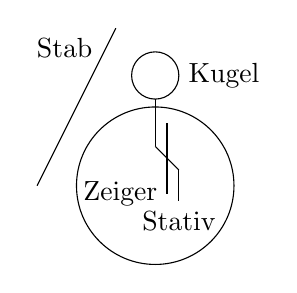
\begin{tikzpicture} 
   \draw (0, 1.4) circle (0.3cm);
   \draw (0.3, 1.4) node [right] {Kugel};
   \draw (0, 0) circle (1cm);
   \draw (0, 1.1) -- (0, 0.5);
   \draw (0, 0.5) -- (0.3, 0.2);
   \draw (0.3, 0.2) -- (0.3, -0.2);
   \draw (0.3, -0.2) node [below] {Stativ};
  
   \draw (0.15, -0.1) -- (0.15, 0.8);
   \draw (0.15, -0.1) node [left] {Zeiger};
   
   \draw (-1.5, 0) -- (-0.5, 2) node [below left, xshift=-5pt] {Stab};
 \end{tikzpicture} 
\end{minipage}
 
 
\end{document}